\documentclass[english,brazil]{ifmgtex}

% ------------------------------------------------------------------------
% Pacotes
% ------------------------------------------------------------------------
% Pacote para destaque de códigos fonte
\usepackage{fancyvrb}

% Pacote para símbulos extras
\usepackage{textcomp}

% Pacote para tabelas
\usepackage{tabularx}

% Algoritmos
\usepackage[noend]{algpseudocode}
% Comandos para traduzir as instruções do pacote de algoritmos
\algrenewcommand\algorithmicrequire{\textbf{Entrada:}}
\algrenewcommand\algorithmicensure{\textbf{Condição:}}
\algrenewcommand\algorithmicend{\textbf{fim}}
\algrenewcommand\algorithmicif{\textbf{se}}
\algrenewcommand\algorithmicthen{\textbf{então}}
\algrenewcommand\algorithmicelse{\textbf{senão}}
\algrenewcommand\algorithmicfor{\textbf{para}}
\algrenewcommand\algorithmicforall{\textbf{para todo}}
\algrenewcommand\algorithmicdo{\textbf{faça}}
\algrenewcommand\algorithmicwhile{\textbf{enquanto}}
\algrenewcommand\algorithmicrepeat{\textbf{repita}}
\algrenewcommand\algorithmicuntil{\textbf{até que}}
\renewcommand{\Return}{\State \textbf{retorne} }

% Comando simples para exibir comandos Latex no texto
\newcommand{\comando}[1]{\textbf{$\backslash$#1}}
\newcommand{\ifmgtex}[1]{IFMG\TeX}

% Estilo de capítulo
% \chapterstyle{bianchi}


% ------------------------------------------------------------------------
% Configurações do Documento
% ------------------------------------------------------------------------
\titulo{IFMG\TeX: Classe {\LaTeX} para Trabalhos Acadêmicos do IFMG}
\autor{Marcos Roberto Ribeiro}
\local{Bambuí - MG}
\data{1}{janeiro}{2017}

\unidade{Campus Bambuí}
% Os possíveis tipos de trabalhos são: monografia, dissertacao ou tese
\tipotrabalho{monografia}
\curso{Bacharel}{Engenharia de Computação}

\areaconcentracao{Processamento de Textos}
% Orientação
\orientador{Nome do Orientador}
\coorientador[Coorientadora]{Nome da Coorientadora}
% Caso o coorientador seja de outra instituição
\coorientadorinstituicao{Instituição da Coorientadora}

% Membros da banca examinadora (além do orientador e coorientador)
\membrobanca{Fulando de Tal}{Instituição do Fulano de Tal}
\membrobanca{Ciclano de Tal}{Instituição do Ciclano de Tal}

% ------------------------------------------------------------------------
% Ficha catalográfica (Obrigatória)
% ------------------------------------------------------------------------
% Caso o comando \fichacatalografica seja definido, a ficha catalográfica
% será inserida no verso da folha de rosto.
% Entre em contato com a biblioteca para obter a ficha catalográfica em
% arquivo PDF. Essa ficha só será inserida no documento após a sua defesa.
\inserirfichacatalografica{ficha_catalografica}

% ------------------------------------------------------------------------
% Folha de aprovação (Obrigatória)
% ------------------------------------------------------------------------
% O comando \inserirfolhaaprovacao{} gera a folha de aprovação para ser
% assinada. Após a defesa esta folha deve ser digitalizada em um arquivo
% PDF e inserida pelo comando \inserirfolhaaprovacao{arquivo}
\inserirfolhaaprovacao{}

% Dedicatória (Opcional)
\inserirdedicatoria{
À minha esposa e ao meu filho.

Aos meus pais e à minha irmã.
}

% Agradecimentos (Opcional)
\inseriragradecimentos{
Agradeço a todos que contribuíram para a realização deste trabalho.
}

% Epígrafe (Opcional)
\inserirepigrafe{
    ``As invenções são, sobretudo, o resultado de um trabalho teimoso.''\\
    (Santos Dumont)
}

\resumo{
  Este trabalho é um breve modelo de trabalho de conclusão de curso utilizando o ambiente Latex.
  Para a confecção deste modelo foi utilizado o pacote de classes \textit{ABNTex} que segue as normas da Associação Brasileira de Normas Técnicas.
  A elaboração de uma monografia pode ser feita sobrescrevendo o conteúdo deste modelo.
}
\palavraschave{Trabalho de Conclusão de Curso. Latex. Monografia.}


% ------------------------------------------------------------------------
% Keywords e abstract
% ------------------------------------------------------------------------
\abstract{
This work is a brief model of course completion work using the Latex environment.
For the preparation of this model was used the package of classes \textit{ABNTex} that follows the norms of the Brazilian Association of Technical Norms.
The elaboration of a monograph can be done by overwriting the content of this model.
}
\keywords{Course Completion Work. Latex. Monograph.}
                % Resumo e Abstract (Obrigatórios)
\inserirlistafiguras                     % Lista de Figuras (Opcional)
\inserirlistaquadros                     % Lista de Quadros (Opcional)
\inserirlistatabelas                     % Lista de Tabelas (Opcional)
\inserirlistaalgoritmos                  % Lista de Algoritmos (Opcional)
\inserirlistacodigos                     % Lista de Códigos (Opcional)
\inserirlistasiglas{\begin{itemize}[]
\item[ABNT] - Associação Brasileira de Normas Técnicas
\item[IFMG] - Instituto Federal de Educação, Ciência e Tecnologia de Minas Gerais
\item[SQL] - \textit{Structured Query Language}
\item[TCC] - Trabalho de conclusão de curso
\end{itemize}
}      % Lista de Siglas (Opcional)
\inserirlistasimbolos{\begin{itemize}[]
  \item $\mathbb{X}$ -- Variável X
  \item $\mathsf{I\!R}$ -- Conjunto dos números reais
\end{itemize}
}  % Lista de Símbolos (Opcional)

\begin{document}

% -----------------------------------------------------------------------------
% Gera elementos pré-textuais
% -----------------------------------------------------------------------------
\maketitle

% -----------------------------------------------------------------------------
% Capítulo: Introdução
% -----------------------------------------------------------------------------
\chapter{Introdução} \label{cap:introducao}

Este documento explica brevemente como trabalhar com a classe \textit{Latex} {IFMG\TeX} para confeccionar trabalhos acadêmicos seguindo as normas da Associação Brasileira de Normas Técnicas (ABNT) e o \textit{Manual de Normalização para Apresentação de Trabalho de Conclusão de Curso} do Instituto Federal Minas Gerais (IFMG) - Campus Bambuí \cite{castro:2016:manual}.
O referido manual foi desenvolvido com o intuito de padronizar as trabalhos acadêmicos produzidos na instituição.

A classe {IFMG\TeX} foi construída com base na classe \textit{abntex2} mantendo as mesmas opções presentes nesta classe, portanto é recomendável que seja consultada a documentação da mesma \cite{araujo:2016:abntex2}.
A classe \textit{abntex2} foi desenvolvida para facilitar a escrita de documentos seguindo as normas da ABNT.
O requisito básico para utilização da classe {IFMG\TeX} é criar um documento com o comando \comando{documentclass\{ifmgtex\}}.
Por padrão, a classe {IFMG\TeX}, cria um documento frente e verso.
Para documentos somente com anverso, é necessário informar a opção \textbf{onseside} (comando \comando{documentclass[oneside]\{ifmgtex\}}).


\chapter{Configuração dos Elementos Pré-Textuais}

A configuração de diversas opções e principalmente dos elementos pré-textuais é realizada com comandos específicos inseridos antes do comando \comando{begin\{document\}}. As informações do documento são configuradas através dos comandos:
\begin{description}
\item[\comando{titulo\{T\}}:] Título do trabalho, substitua T pelo título do trabalho;
% ------------------------------------------------------------------------
\item[\comando{autor\{N\}}:] Nome do autor do trabalho;
% ------------------------------------------------------------------------
\item[\comando{local\{L\}}:] Local do trabalho;
% ------------------------------------------------------------------------
\item[\comando{data\{dia\}\{mês (por extenso)\}\{ano\}}:] Configuração da data do documento que aparecerá na folha de aprovação;
% ------------------------------------------------------------------------
\item[\comando{unidade\{U\}}:] Nome da unidade do IFMG, por exemplo, Campus Bambuí;
% ------------------------------------------------------------------------
\item[\comando{tipotrabalho\{T\}}:] Tipo de trabalho, os possíveis tipos de trabalhos são: monografia, dissertacao ou tese;
% % ------------------------------------------------------------------------
\item[\comando{curso\{NC\}\{TC\}}:] Dados do curso, nome do curso(NC) e grau obtido com o curso(GC).
Exemplo: \comando{curso\{Bacharel\}\{Engenharia de Computação\}\{Bacharel\}};
% ------------------------------------------------------------------------
\item[\comando{areaconcentracao\{T\}}:] Área de concentração do trabalho;
% ------------------------------------------------------------------------
\item[\comando{orientador\{O\}}:] Nome do professor orientador do trabalho.
Caso seja uma orientadora pode ser usado o comando \comando{orientador[Orientadora]\{O\}};
% ------------------------------------------------------------------------
\item[\comando{coorientador\{C\}}:] Nome do coorientador do trabalho.
Caso seja uma coorientadora pode ser usado um comando análogo a definição de orientadora como \comando{coorientador[Coorientadora]\{C\}}.
No caso de coorientadores de outras instituições, é preciso usar  comando \comando{coorientadorinstituicao\{I\}}, onde I é a instituição do coorientador;
% ------------------------------------------------------------------------
\item[Membros da banca avaliadora:] Os membros da banca avaliadora constarão na folha de aprovação juntamente com os nomes do orientador e do coorientador.
A definição dos membros é feita com o comando \comando{membrobanca\{N\}\{I\}}, onde N é o nome do membro e I é sua instituição.
é preciso usar um comando para cada membro;
% ------------------------------------------------------------------------
\item[\comando{inserirfichacatalografica\{F\}}:] Insere a ficha catalográfica (elemento obrigatório) contida no arquivo F\footnote{A ficha catalográfica é inserida apenas em documentos frente e verso.}.
Entre em contato com a biblioteca para obter a ficha catalográfica em arquivo PDF.
Essa ficha deverá ser inserida no documento após a defesa;
% ------------------------------------------------------------------------
\item[\comando{inserirfolhaaprovacao\{F\}}:] Insere a folha de aprovação (elemento obrigatório).
O comando \comando{inserirfolhaaprovacao\{\}} gera a folha de aprovação para ser assinada.
Após a defesa esta folha deve ser digitalizada para um arquivo PDF e inserida pelo comando \inserirfolhaaprovacao{arquivo};
% ------------------------------------------------------------------------
\item[Dedicatória, Agradecimentos e Epígrafe:] Os elementos pré-textuais opcionais dedicatória, agradecimentos e epígrafe são inseridos com os comandos \comando{inserirdedicatoria\{T\}}, \comando{inseriragradecimentos\{T\}} e \comando{inserirepigrafe\{T\}}, respectivamente.
é preciso usar um comando para cada membro;
% ------------------------------------------------------------------------
\item[Resumo e \textit{Abstract}:] O resumo é incluído com o comando \comando{resumo\{T\}}. Este comando deve ser imediatamente seguido pelo comando \comando{palavraschave\{P\}} para definição das palavras chaves, sendo que P são as palavras chaves iniciando com letras maiúsculas e separadas por pontos. O \textit{Abstract} é configurado de forma análoga com os comandos \comando{abstract\{T\}} e \comando{keywords\{K\}}.
% ------------------------------------------------------------------------
\item[\comando{inserirlistafiguras}:] Insere a lista de figuras;
% ------------------------------------------------------------------------
\item[\comando{inserirlistaquadros}:] Insere a lista de quadros;
% ------------------------------------------------------------------------
\item[\comando{inserirlistatabelas}:] Insere a lista de tabelas;
% ------------------------------------------------------------------------
\item[\comando{inserirlistaalgoritmos}:] Insere a lista de algoritmos;
% ------------------------------------------------------------------------
\item[\comando{inserirlistacodigos}:] Insere a lista de códigos;
% ------------------------------------------------------------------------
\item[\comando{inserirlistasiglas\{L\}}:] Insere a lista de siglas. O parâmetro L é a própria lista de siglas definida em um ambiente \textit{itemize} como mostrado no Código \ref{codigo:lista_siglas};
% ------------------------------------------------------------------------
\item[\comando{inserirlistasimbolos\{L\}}:] Insere a lista de siglas. O parâmetro L é a definição da lista de símbolos de forma análoga a definição da lista de siglas.
\end{description}

\begin{codigo}[!htb]
\begin{Verbatim}
\begin{itemize}[]
\item[ABNT] - Associação Brasileira de Normas Técnicas
\item[IFMG] - Instituto Federal Minas Gerais
\item[SQL] - \textit{Structured Query Language}
\item[TCC] - Trabalho de conclusão de curso
\end{itemize}
\end{Verbatim}
\caption{Lista de siglas} \label{codigo:lista_siglas}
\end{codigo}


\chapter{Corpos Flutuantes}

Corpos flutuantes são elementos não textuais como figuras e tabelas que complementam as informações do texto. Neste capítulo são expostos breves exemplos dos corpos flutuantes disponíveis na classe {IFMG\TeX}.

Na Seção \ref{secao:figuras} é mostrado como inserir figuras, a Seção \ref{secao:tabelas_e_quadros} explica como incluir tabelas e quadros e a Seção \ref{secao:algoritmos_e_codigos} demostra como trabalhar com algoritmos e códigos fontes.

\section{Figuras}
\label{secao:figuras}

A inserção de figuras é realizada normalmente através do comando \comando{begin\{figure\}}. A Figura \ref{figura:logomarca_ifmg} exibe a logomarca do IFMG. De acordo com as normas ABNT a lista de figuras é um elemento opcional do documento, para incluí-la é preciso inserir o comando \comando{inserirlistafiguras} antes do início do documento.

\begin{figure}[htb]
 \centering
 \iflogo
 \caption{Logomarca do IFMG}
 \label{figura:logomarca_ifmg}
\end{figure}

\section{Tabelas e Quadros}
\label{secao:tabelas_e_quadros}

A inserção de tabelas e quadros é feita de forma semelhante a inserção de figuras, porém são utilizados os ambientes \textit{table} e \textit{quadro}. A principal diferença entre tabelas e quadros, de acordo com \citet{castro:2016:manual}, é que as tabelas são destinadas para informações numéricas e os quadros são mais adequados para informações textuais.

Como exemplos foram inseridas a Tabela \ref{tabela:lista_produtos} que exibe uma de lista de produtos e a Tabela \ref{tabela:populacao_america_sul} que mostra a população dos países da América do Sul. Foi inserido também o Quadro \ref{quadro:editores_texto_livres} com alguns editores que podem ser usados para se trabalhar com Latex para demonstrar a inserção de quadros.

 A lista de tabelas também é um elemento opcional que pode ser incluída com o comando \comando{inserirlistatabelas} antes do início do documento. O mesmo acontece com a lista de quadros que pode ser incluída com o comando \comando{inserirlistaquadros}.

\begin{table}[htb]
\centering
\caption{Lista de produtos}
\label{tabela:lista_produtos}
\begin{tabularx}{\textwidth}{X|l|r|r|r} \hline
Produto      & Unidade & Preço (R\$) & Quantidade & Total (R\$) \\ \hline
Arroz        & Kg      & 2,00        & 550        & 1.100,00    \\
Óleo de Soja & L       & 2,50        & 500        & 750,00      \\
Açucar       & Kg      & 3,00        & 100        & 300,00      \\ \hline
\end{tabularx}
\end{table}

\begin{table}[htb]
\centering
\caption{População dos países da América do Sul} \label{tabela:populacao_america_sul}
\begin{tabular}{r|l|r}        \hline
Código  & País            & População   \\ \hline
1       & Brasil          & 191.480.630 \\
2       & Argentina       &  39.934.100 \\
3       & Colômbia        &  46.741.100 \\
4       & Paraguai        &   9.694.200 \\
5       & Uruguai         &   3.350.500 \\
6       & Peru            &  28.221.500 \\
7       & Equador         &  13.481.200 \\
8       & Bolívia         &   9.694.200 \\
9       & Venezuela       &  28.121.700 \\
10      & Chile           &  16.803.000 \\ \hline
\end{tabular}

\begin{small}
Fonte: \citeonline{wikipedia:2011:america_sul}.
\end{small}
\end{table}

\begin{quadro}[htb]
\centering
\begin{tabular}{|l|l|r|}        \hline
Editor     & Multiplataforma & Específico para Latex \\ \hline
Kwriter    & Sim             & Não                   \\
Texmaker   & Sim             & Sim                   \\
Kile       & Sim             & Sim                   \\
Geany      & Sim             & Não                   \\ \hline
\end{tabular}
\caption{Editores de Texto Livres}
\label{quadro:editores_texto_livres}
\end{quadro}

\section{Algoritmos e Códigos} \label{secao:algoritmos_e_codigos}

Além dos corpos flutuantes convencionais para inserir figuras (\comando{begin\{figure\}}) e tabelas (\comando{begin\{figure\}}), a classe {IFMG\TeX} possui mais dois tipos de corpos flutuantes um para algoritmos (\comando{begin\{algoritmo\}}) e outro para códigos (\comando{begin\{codigo\}}). Como exemplo temos o Algoritmo \ref{algoritmo:mdc} que calcula o máximo divisor comum entre dois números e os Códigos \ref{codigo:notas_alunos} e \ref{codigo:metodo_leitura} que são uma consulta na \textit{Structured Query Language (SQL)} e um método em Java que recebe um texto digitado pelo usuário, respectivamente.

\begin{algoritmo}[!htb]
\begin{algorithmic}[1]
 \Require Dois números inteiros ($n_1, n_2$)
 \If{$n_2 > n_1$} \Comment{Garante que o maior número seja $n_1$}
   \State troca valores de $n_1$ e $n_2$
 \EndIf
 \Repeat
   \State $r \leftarrow$ resto da divisão de $n_1$ por $n_2$
   \State $n_1 \leftarrow n_2$
   \State $n_2 \leftarrow r$
 \Until{$r > 0$}
 \Return $n_1$
\end{algorithmic}
\caption{Algoritmo para cálculo de máximo divisor comum MDC($n_1$,$n_2$)}
\label{algoritmo:mdc}
\end{algoritmo}

\begin{codigo}[!htb]
\begin{Verbatim}
SELECT a.nome_aluno AS aluno,
       d.nome_disciplina AS disciplina,
       m.nota AS nota
FROM aluno AS a,
     disciplina AS d,
     matriculado AS m
WHERE a.id_aluno = m.id_aluno
  AND d.id_disciplina = m.id_disciplina
ORDER BY a.nome_aluno, d.nome_disciplina;
\end{Verbatim}
\caption{Consulta SQL} \label{codigo:notas_alunos}
\end{codigo}

\begin{codigo}[!htb]
\begin{Verbatim}
public static String Leitura(){
    BufferedReader reader =
        new BufferedReader(new InputStreamReader(System.in));
    try {
        return reader.readLine(); // Lê uma linha pelo teclado
    } catch (IOException e) {
        e.printStackTrace();
        return "";
    }
}
\end{Verbatim}
\caption{Sub-rotina para obter uma entrada do usuário} \label{codigo:metodo_leitura}
\end{codigo}

Existem diversos outros pacotes disponíveis para escrever algoritmos e códigos. Nos exemplos anteriormente foram utilizados o pacote \textit{algpseudocode} e \textit{fancyvrb}. O pacote \textit{algpseudocode} é usado para escrever algoritmos em alto nível \cite{janos:2005:algpseudocode}. Já o pacote \textit{fancyvrb} serve para escrever códigos mono-espaçados \cite{zandt:2010:fancyvrb}.
Caso sejam utilizados os ambientes de algoritmo e código, podem ser incluídos os comandos \comando{inserirlistaalgoritmos} e \comando{inserirlistacodigos} antes do \comando{begin\{document\}} para que a lista de algoritmos e a lista de código sejam criadas.
Existem também diversos outros pacotes para formatação de algoritmos e códigos que podem ser usados como o \textit{minted} com suporte a diversas linguagens de programação \cite{poore:2016:minted}.


\chapter{Ambientes Matemáticos}

A classe {IFMG\TeX} provê os seguintes ambientes matemáticos:
\begin{itemize}
 \item Teoremas (\comando{begin\{teorema\}[\ ]} ... \comando{begin\{teorema\}});
 \item Proposição (\comando{begin\{proposicao\}[\ ]} ... \comando{begin\{proposicao\}});
 \item Lema (\comando{begin\{lema\}[\ ]} ... \comando{begin\{lema\}});
 \item Corolário (\comando{begin\{corolario\}[\ ]} ... \comando{begin\{corolario\}});
 \item Exemplo (\comando{begin\{exemplo\}[\ ]} ... \comando{begin\{exemplo\}});
 \item Observação (\comando{begin\{observacao\}[\ ]} ... \comando{begin\{observacao\}});
 \item Definição (\comando{begin\{definicao\}[\ ]} ... \comando{begin\{definicao\}});
 \item demonstracao (\comando{begin\{demonstracao\}[\ ]} ... \comando{begin\{demonstracao\}}).
\end{itemize}

Abaixo temos um exemplo de proposição com sua demonstração:
\begin{proposicao}
 Sejam $a$ e $b$ reais, tais que $0<a<b$. Então $a^2<b^2$.
\end{proposicao}
\begin{demonstracao}
 Pela hipótese concluímos que $(b+a)>0$ e $(b-a)>0$.

Como $b^2-a^2=(b+a)(b-a)$ concluímos que $b^2-a^2>0$, ou seja, $a^2<b^2$.
\end{demonstracao}

Neste documento tratamos brevemente apenas dos ambientes mencionados anteriormente. Contudo, para escrever expressões matemáticas complexas é preciso estudar uma documentações mais específicas\footnote{\url{https://en.wikibooks.org/wiki/LaTeX/Mathematics}}\footnote{\url{https://en.wikibooks.org/wiki/LaTeX/Advanced_Mathematics}}.
Alguns dos ambientes matemáticos da classe {IFMG\TeX} podem ser usados também para outras finalidades como exemplos e definições.


\chapter{Ferramentas Úteis} \label{capitulo:ferramentas_uteis}

Existem diversas ferramentas para se trabalhar com Latex. Duas ferramentas que merecem destaque são o editor \textit{Texmaker} exibido na Figura \ref{figura:texmaker} e o gerenciador de referências \textit{JabRef} mostrado na Figura \ref{figura:jabref}. Ambas ferramentas são livres e multiplataforma.

\begin{figure}[htb]
 \centering
 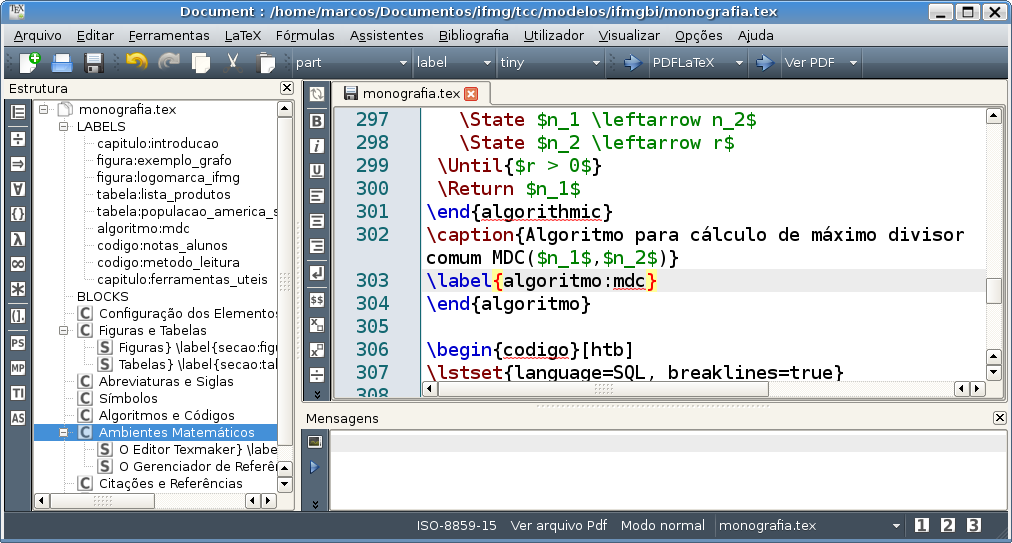
\includegraphics[width=\textwidth]{figuras/texmaker}
 \caption{Tela do Texmaker}
 \label{figura:texmaker}
\end{figure}

\begin{figure}[htb]
 \centering
 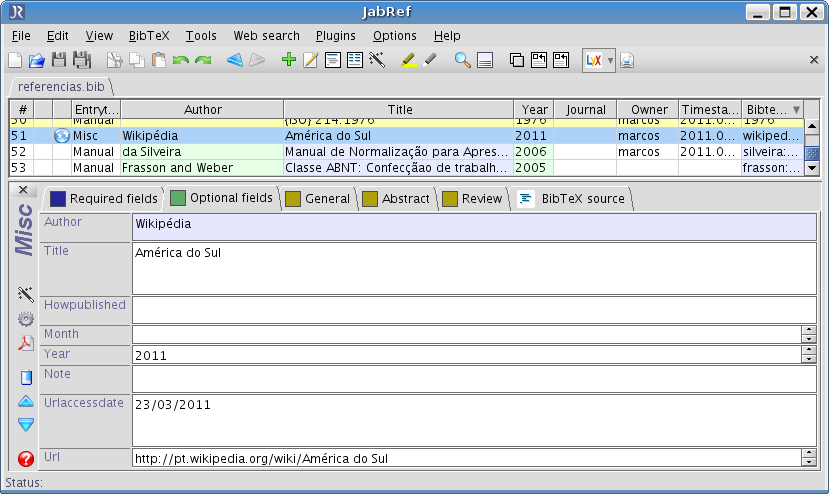
\includegraphics[width=\textwidth]{figuras/jabref}
 \caption{Tela do JabRef}
 \label{figura:jabref}
\end{figure}

O Texmaker pode ser obitido em \url{http://www.xm1math.net/texmaker} e o JabRef pode ser obtido em \url{http://www.jabref.org/}. É importante ressaltar que o Texmaker é apenas um editor, para compilar os documentos é necessário um ambiente Latex instalado. Os ambientes Latex mais populares são o Texlive (\url{http://www.tug.org/texlive}) e o MiKTex (\url{http://miktex.org}).


\chapter{Citações e Referências}

Em documentos acadêmicos podem existir citações diretas e citações indiretas. As citações indiretas são feitas quando se reescreve uma referência consultada. Nas citações indiretas há duas formatações possíveis dependendo de como ocorre a citação no texto. Quando o autor é mencionado explicitamente na sentença deve ser usado o comando \comando{citet\{\}}, nas demais situações é usado o comando \comando{cite\{\}}. A Figura \ref{figura:citacao_indireta_explicita} mostra um exemplo com o comando \comando{citet\{\}}.

\begin{figure}[htb]
\hrulefill

\begin{verbatim}
Segundo \citet{castro:2016:manual}, o trabalho de conclusão de curso
deve seguir as normas da ABNT.
\end{verbatim}

\hrulefill

Segundo \citet{castro:2016:manual}, o trabalho de conclusão de curso deve seguir as normas da ABNT.

\hrulefill

\caption{Exemplo de citação indireta explícita} \label{figura:citacao_indireta_explicita}
\end{figure}

Para especificar a página consultada na referência é preciso acrescentá-la entre colchetes com os comandos \comando{cite[página]\{\}} ou \comando{citet[página]\{\}}. Na Figura \ref{figura:citacao_indireta_pagina} é mostrado um exemplo de citação com página específica.

\begin{figure}[htb]
\hrulefill

\begin{verbatim}
A folha de aprovação é um elemento obrigatório no trabalho de conclusão
de curso \cite[p.~22]{castro:2016:manual}.
\end{verbatim}

\hrulefill

A folha de aprovação é um elemento obrigatório no trabalho de conclusão de curso \cite[p.~22]{castro:2016:manual}.

\hrulefill

\caption{Exemplo de citação indireta não explícita} \label{figura:citacao_indireta_pagina}
\end{figure}

As citações diretas acontecem quando o texto de uma referência é transcrito literalmente. As citações diretas são curtas (até três linhas) são inseridas no texto entre aspas duplas. Como no exemplo mostrado na Figura \ref{figura:citacao_direta_curta}.

\begin{figure}[htb]
\hrulefill

\begin{verbatim}
``A tabela deve ser colocada em posição vertical, para facilitar a
leitura dos dados'' \cite[p.~26]{castro:2016:manual}.
\end{verbatim}

\hrulefill

``A tabela deve ser colocada em posição vertical, para facilitar a leitura dos dados'' \cite[p.~25]{castro:2016:manual}.

\hrulefill

\caption{Exemplo de citação direta curta}
\label{figura:citacao_direta_curta}
\end{figure}

As citações longas (com mais de 3 linhas) podem ser inseridas com o ambiente \comando{begin\{citacao\}} como mostra a Figura \ref{figura:citacao_direta_longa}.

\begin{figure}[htb]
\hrulefill

\begin{verbatim}
\begin{citacao}
A tabela deve ser colocada em posição vertical, para facilitar a
leitura dos dados.
No caso em que isso seja impossível, deve ser colocada em posição
horizontal, com o título voltado para a margem esquerda da folha.
Fontes e notas devem aparecer na parte inferior da
tabela em tamanho 11 \cite[p.~25]{castro:2016:manual}.
\end{citacao}
\end{verbatim}

\hrulefill

\begin{citacao}
A tabela deve ser colocada em posição vertical, para facilitar a leitura dos dados. No
caso em que isso seja impossível, deve ser colocada em posição horizontal, com o título
voltado para a margem esquerda da folha. Fontes e notas devem aparecer na parte inferior da
tabela em tamanho 11 \cite[p.~25]{castro:2016:manual}.
\end{citacao}

\hrulefill

\caption{Exemplo de citação direta longa}
\label{figura:citacao_direta_longa}
\end{figure}


% -----------------------------------------------------------------------------
% Elementos pós-textuais
% -----------------------------------------------------------------------------
\postextual

% -----------------------------------------------------------------------------
% Referências bibliográficas
% -----------------------------------------------------------------------------
\bibliography{referencias}

% -----------------------------------------------------------------------------
% Apêndices
% -----------------------------------------------------------------------------
\apendices\partapendices

\chapter{Documento Básico Usando a Classe {IFMG\TeX}}

\begin{Verbatim}[frame=single, fontsize=\scriptsize]
\documentclass[english,brazil]{ifmgtex} % Documento utilizando a classe ifmgtex

\titulo{Título do trabalho}         % Título
\autor{Nome do Autor}               % Autor
\instituicao{Instituto Federal de Educação, Ciência e Tecnologia de Minas Gerais - Campus
Bambuí}                      % Instituição
\local{Bambuí - MG}                 % Local
\data{1}{junho}{2017}               % Data da defesa

\unidade{Campus Bambuí}             % Unidade do IFMG
\tipotrabalho{monografia}           % monografia, dissertacao ou tese
\curso{Bacharel}{Engenharia de Computação}  % Título obtido e Curso

\areaconcentracao{Processamento de Textos}   % Área de concentração
\orientador{Nome do Orientador}              % Orientador
\coorientador[Coorientadora]{Nome da Coorientadora}     % Coorientadora
\coorientadorinstituicao{Instituição da Coorientadora}

% Membros da banca examinadora (além do orientador e coorientador)
\membrobanca{Fulando de Tal}{Instituição do Fulano de Tal}
\membrobanca{Ciclano de Tal}{Instituição do Ciclano de Tal}

\inserirfichacatalografica{ficha_catalografica} % Ficha catalográfica
\inserirfolhaaprovacao{}                        % Folha de aprovação

\inserirdedicatoria{
  Texto da dedicatória.
}

\inseriragradecimentos{
  Texto dos agradecimentos.
}

\inserirepigrafe{
  ``As invenções são, sobretudo, o resultado de um trabalho teimoso.''\\
  (Santos Dumont)
}

\resumo{
  Texto do resumo.
}
\palavraschave{Palavras. Chave;}

\abstract{
  Texto do abstract.
}
\keywords{English. Keywords.}

\inserirlistafiguras                     % Lista de Figuras
\inserirlistaquadros                     % Lista de Quadros
\inserirlistatabelas                     % Lista de Tabelas
\inserirlistaalgoritmos                  % Lista de Algoritmos
\inserirlistacodigos                     % Lista de Códigos
\inserirlistasiglas{\begin{itemize}[]
\item[ABNT] - Associação Brasileira de Normas Técnicas
\item[IFMG] - Instituto Federal de Educação, Ciência e Tecnologia de Minas Gerais
\item[SQL] - \textit{Structured Query Language}
\item[TCC] - Trabalho de conclusão de curso
\end{itemize}
}      % Lista de Siglas
\inserirlistasimbolos{\begin{itemize}[]
  \item $\mathbb{X}$ -- Variável X
  \item $\mathsf{I\!R}$ -- Conjunto dos números reais
\end{itemize}
}  % Lista de Símbolos

% Início do documento
\begin{document}

\maketitle

\chapter{Introdução}

Capítulo de Introdução

\chapter{Desenvolvimento}

Capítulo de Desenvolvimento

\chapter{Conclusão}

Capítulo de conclusão

\postextual

\bibliography{referencias}

\apendices\partapendices

\chapter{Título do Apêndice}

Conteúdo do apêndice

\anexos\partanexos

\chapter{Título do Anexo}

Conteúdo do anexo.

\end{document}
\end{Verbatim}


% -----------------------------------------------------------------------------
% Anexos
% -----------------------------------------------------------------------------
\anexos\partanexos

\chapter{Páginas Interessantes na Internet} \label{capitulo:paginas_interessantes}

\begin{description}
 \item[\url{http://en.wikibooks.org/wiki/LaTeX}:] Livro em formato \textit{wiki} gratuito sobre {\LaTeX} (possui uma versão em português, mas a versão em inglês é a mais completa);
 \item[\url{http://tobi.oetiker.ch/lshort/lshort.pdf}:] Ótimo tutorial sobre {\LaTeX};
 \item[\url{abntex.codigolivre.org.br}:] Página do projeto \textit{abnTeX2} com informações sobre os pacotes e classes em {\LaTeX} para as normas da ABNT, nos quais a classe {IFMG\TeX} foi baseada.
\end{description}


\end{document}
